\documentclass{asaproc}
%\documentclass{article}
\usepackage{amssymb,amsmath,amsthm}
\usepackage{graphicx}
%\usepackage[ruled,linesnumbered]{algorithm2e}
\usepackage[caption = false]{subfig}
\usepackage{float}
\usepackage{hyperref}

%\usepackage{times}
%If you have times installed on your system, please
%uncomment the line above

%For figures and tables to stretch across two columns
%use \begin{figure*} \end{figure*} and
%\begin{table*}\end{table*}
% please place figures & tables as close as possible
% to text references

% Commands
\newcommand{\sq}{\sigma^2}
\newcommand{\tq}{\tau^2}
\newcommand{\laq}{\lambda^2}
\newcommand{\bh}{\hat{\beta}}
\newcommand{\Sh}{\hat{\Sigma}}

% Figures Path
\graphicspath{{./figures/}}

\title{Defending Against Adversarial Attacks}

%input all authors' names

\author{Keller Jordan, Rene Gutierrez \& Brett G\"{o}hre \\}

%input affiliations

%{USDA Forest Service Forest Products Laboratory}

\begin{document}

\maketitle


\begin{abstract}

Adversarial attacks have been a growing concern as the success of Neural Networks has increased. To address this issue, in this project we explore a variety of techniques to defend against such attacks. To defend against black-box attacks, we use attempt to use Random Compression Matrices. For white-box attacks, we compare the robustness of the exponentiated gradient optimization scheme to classic stochastic gradient descent. And for an encoder-decoder architecture where the encoder is attacked in a white-box scenario without access to the decoder, we investigate reconstruction-error based detection.
	
\begin{keywords}
Adversarial Examples, White-Box Attacks, Black-Box Attacks, Random Projection Matrix, Reconstruction Error, Capsule Networks, Convolutional Neural Networks.
\end{keywords}
\end{abstract}


\section{Introduction}

There is an increasing concern that Neural Networks are very susceptible to Black Box Adversarial Attacks, with implications that go from identity theft, as in biometrics recognition to safety in the self-driving car industry. So it is of the utmost importance to try to create defenses against such attacks, or at the very least study their characteristics. Here we try several alternatives with varying degrees of success, however even in failure, new insights are gained in exploration.

\section{Random Projection Matrices}

\subsection*{Idea}

Random compression matrices have been found to be able to perform dimensionality reduction exploiting the input data structure, in particular when the data could belong to a manifold. We can make further use of this in two ways, first the dimensionality reduction can help create smaller models that could help robustness. Furthermore, the random nature of the matrix can transform the attack and make it less or not powerful at all.

\subsection*{Method}

For this idea we worked with the MNIST dataset. First, we created 2 sets of adversarial examples based on different architectures. The first set was based on Logistic Regression and consists of 758 adversarial images. The second one was based on a Convolutional Neural Network optimized to 95\% accuracy in the validation set, and had 440 adversarial images. Then we tried to attack these architectures plus a Random Compression Matrix architecture, a Random Expansion Matrix and 2 CNN optimized to 90\% and 99\% accuracy.

The Random Projection architectures where basically a Logistic Regression for which a Random Projection Matrix $ \Phi $ is applied to the input $ x $, but remains fixed through training. The idea was that since adversarial attacks are based on small perturbations $ \epsilon $ to the input, then when applying the random matrix the perturbation would be rendered meaningless, that is $ \Phi \epsilon $ would not be able to attack as effectively. Furthermore, since the attacker would not know $ \Phi $, it would not be able to train attacks specific to it. In this way our random projection matrix can be thought as some kind of code.

\begin{figure}[h!]
	\centering
	\caption{\enspace Examples of the Adversarial Attacks created under the 2 Architectures. The top row shows the attacks created with the Logistic Regression, while the bottom was created using a CNN.}
	\subfloat[Adversarial Attack for 3]{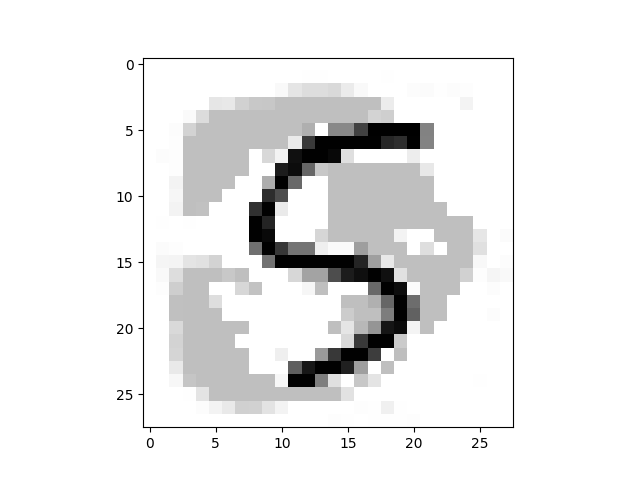
\includegraphics[width=0.45\linewidth]{advImg.png}} 
	\subfloat[Noise  ]{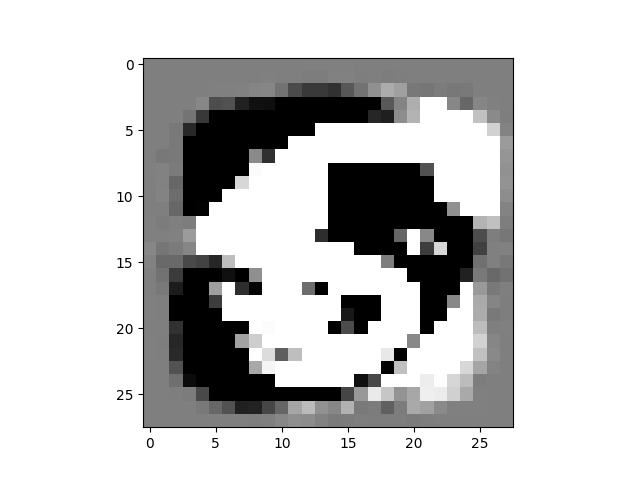
\includegraphics[width=0.45\linewidth]{advNoi.png}}   \\
	\subfloat[Adversarial Attack for 3]{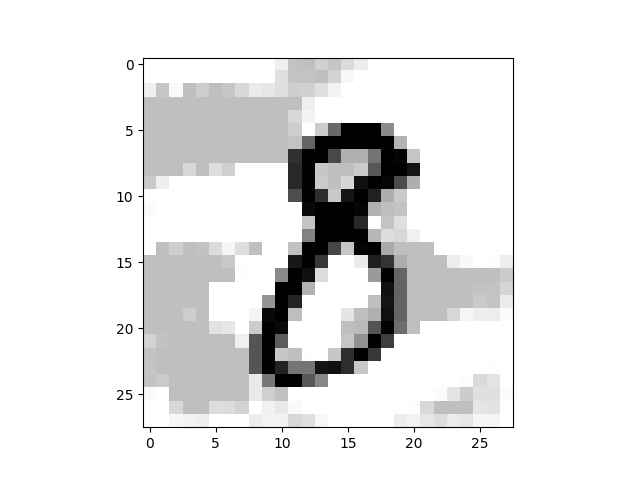
\includegraphics[width=0.45\linewidth]{advImgCnn.png}} 
	\subfloat[Noise  ]{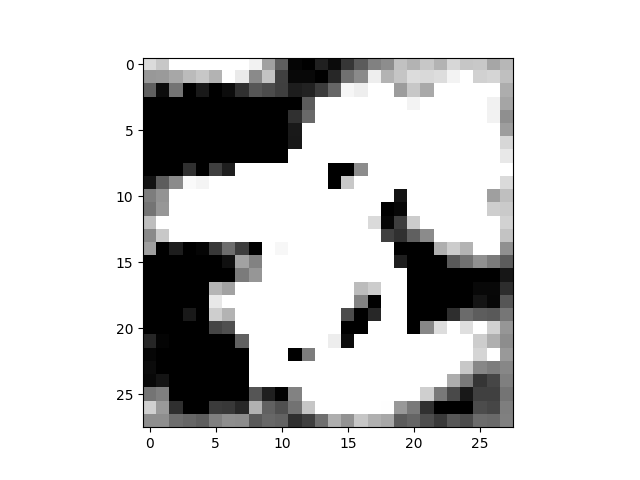
\includegraphics[width=0.45\linewidth]{advNoiCnn.png}}   \\
	\label{fig1}
\end{figure}


\subsection*{Results}

\begin{table*}
	\caption{\enspace Accuracy for the 5 different methods, using the test set and the adversarial examples generated by Logistic Regression and CNN architectures.}
	\label{tab1}
	\begin{tabular*}{\hsize}{@{\extracolsep{\fill}}cccc}
		\hline
		\\[-7pt]
		\multicolumn{1}{c}{\it Method}                    & 
		\multicolumn{1}{c}{\it Test Set}                  & 
		\multicolumn{1}{c}{\it Logistic Arch Adversarial} & 
		\multicolumn{1}{c}{\it CNN Arch Adversarial}      \\
		\hline
		\\[-5pt]
		Logistic Regression      & 92.00\% & 0.00\%  & 3.41\%  \\
		CNN 90\%                 & 89.82\% & 8.71\%  & 5.23\%  \\
		CNN 95\%                 & 94.64\% & 9.50\%  & 9.50\%  \\
		CNN 99\%                 & 98.63\% & 60.95\% & 11.36\% \\
		Compression Logistic to 196 dim & 89.56\% & 0.00\%  & 5.00\%  \\
		Expansion Logistic to 1960 dim  & 91.07\% & 0.00\%  & 3.64\% 
	\end{tabular*}
\end{table*}

\begin{figure}[h!]
	\centering
	\caption{\enspace Confusion Matrices for the True Target and Predicted Target on the Left and the Adversarial Target and Predicted Target on the Right. The top row shows the results using the a compression matrix, while the bottom row shows the results on an expansion matrix. Both results are for the adversarial examples generated with the Logistic Regression architecture.}
	\subfloat[Confusion Matrix for True Class]{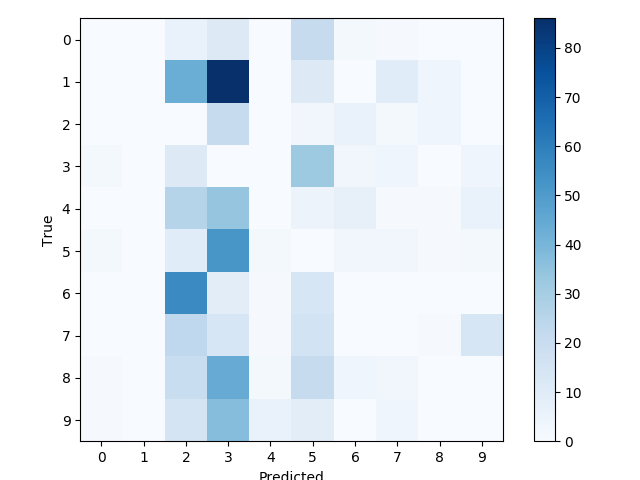
\includegraphics[width=0.5\linewidth]{confussionMatrixAdvTrueCom.png}} 
	\subfloat[Confusion Matrix for Target Class]{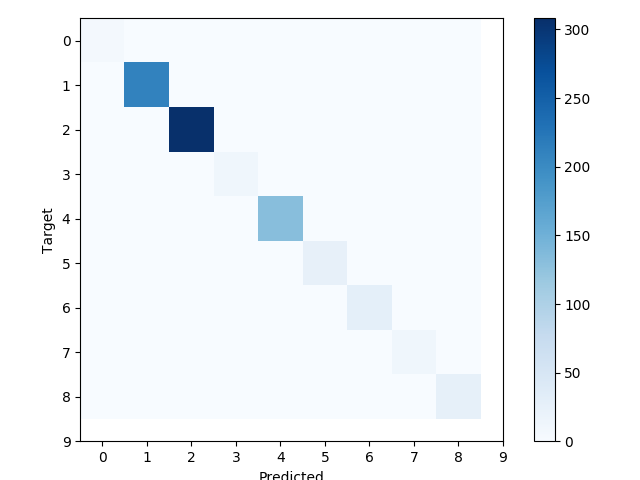
\includegraphics[width=0.5\linewidth]{confussionMatrixAdvTarCom.png}}   \\
	\subfloat[Confusion Matrix for True Class]{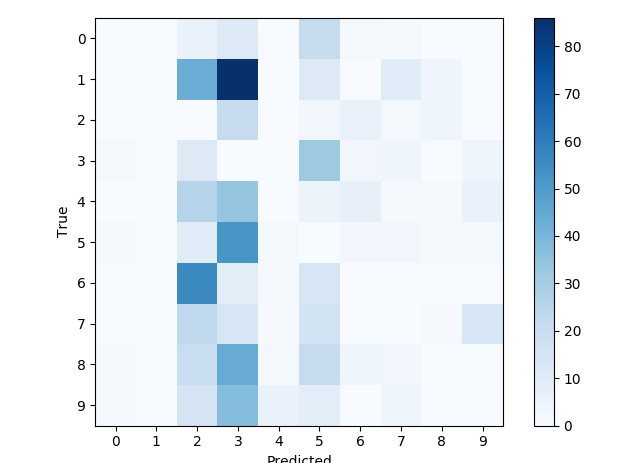
\includegraphics[width=0.5\linewidth]{confussionMatrixAdvTrueExp.png}} 
	\subfloat[Confusion Matrix for Target Class]{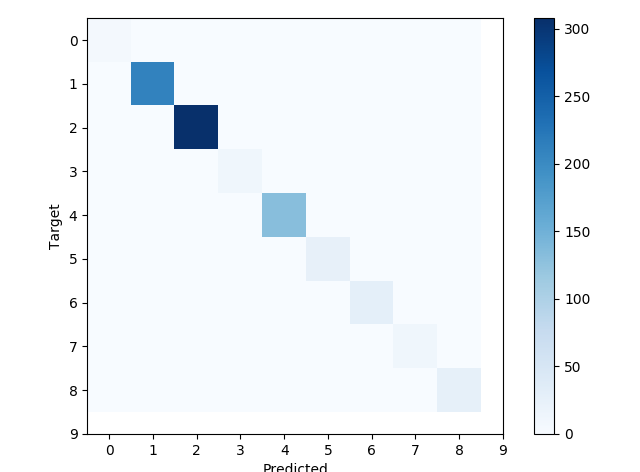
\includegraphics[width=0.5\linewidth]{confussionMatrixAdvTarExp.png}}   \\
	\label{fig2}
\end{figure}

In figure \ref{fig2} we can see the corresponding confusion matrices for the true class on the left and for the adversarial class on the right for the examples generated from the Logistic regression architecture. As we can see the adversarial attacks not only make the expansion and compression defenses fail to predict correctly, but are completely fooled by the examples.

Furthermore, in table \ref{tab1} we can see that the adversarial examples generated by different architectures transfer successfully across architectures. Even fooling completely the randomness induced by the projecting matrices. However it seems that training the CNN to until it achieves higher accuracy provides the best protection, however it still performs poorly and offers little protection for examples generated on the CNN.

To analyze the weights obtained after compression and expansion, and compared them to the weights obtained under regular logistic regression, we apply the pseudo inverse of the projection matrix $ \Phi^+ $. In figure \ref{fig4} we can see the weights re-expanded or re-compressed to the original size. The weights for the Expansion weights are very close to the regular weights, so it comes as no surprise that the Expansion Logistic Regression fails to defend against adversarial attacks. However, even though the weights from the Compressed Logistic are significantly different this did not prevent it from getting fooled. Also, the weights seem to converge to the regular weights as the level of compression decreases, as we can see in figure \ref{fig5}, giving us a hint of why the network still gets fooled.

\begin{figure}[h!]
	\centering
	\caption{\enspace Weights for "Neuron 2", for the Compression, Expansion and Regular Logistic Regression.}
	\subfloat[Compression]{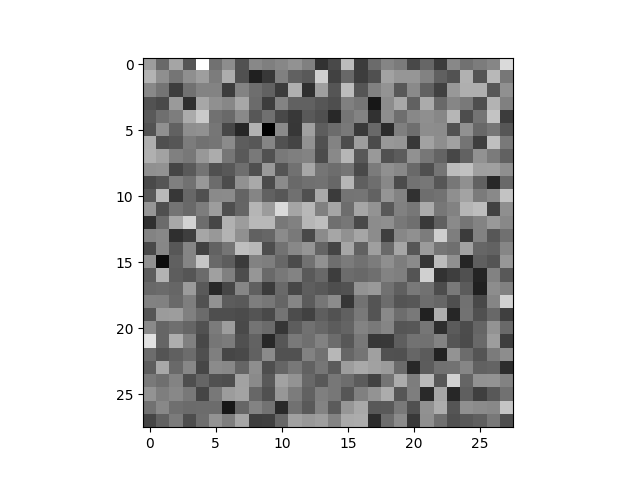
\includegraphics[width=0.33\linewidth]{com2.png}}
	\subfloat[Expansion]{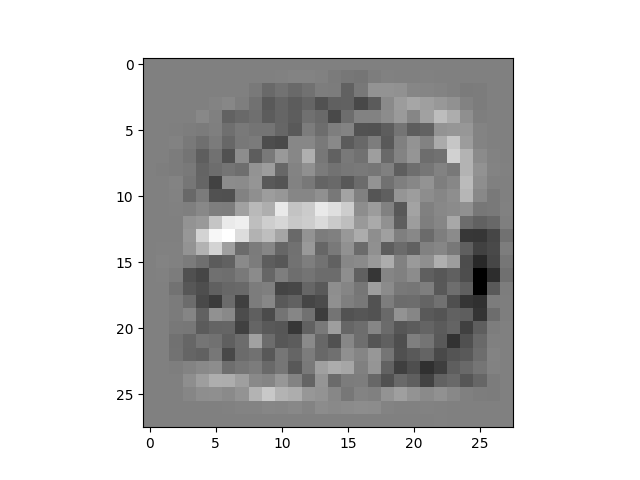
\includegraphics[width=0.33\linewidth]{exp2.png}}
	\subfloat[Regular]{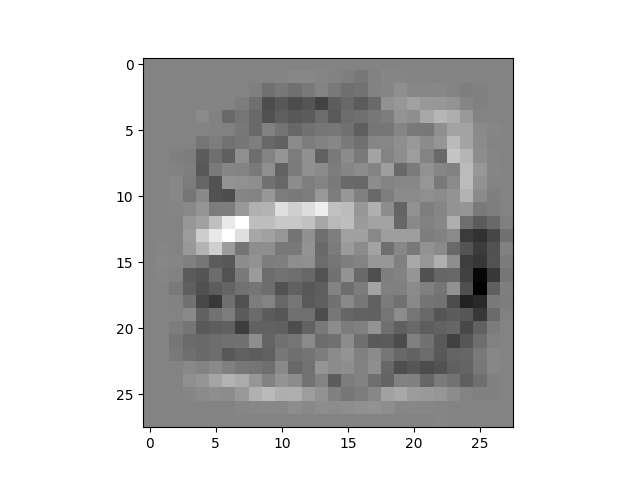
\includegraphics[width=0.33\linewidth]{reg2.png}}
	\label{fig4} 
\end{figure}

\begin{figure}[h!]
	\centering
	\caption{\enspace Weights for 2, for the Compression t0 196, Compression to 392, Compression to 588 and Regular Logistic Regression.}
	\subfloat[196]{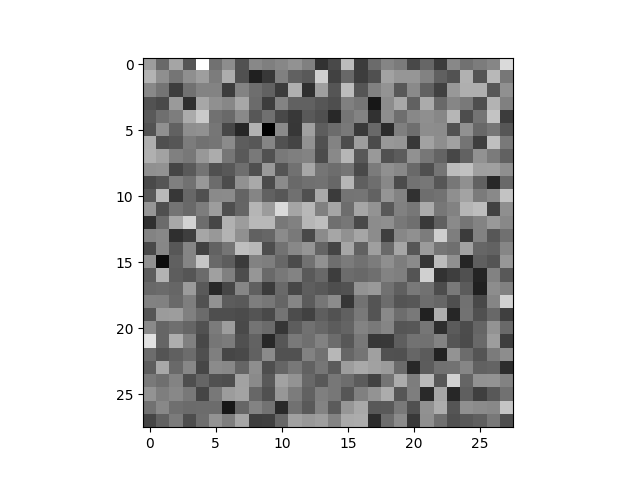
\includegraphics[width=0.25\linewidth]{com2.png}}
	\subfloat[392]{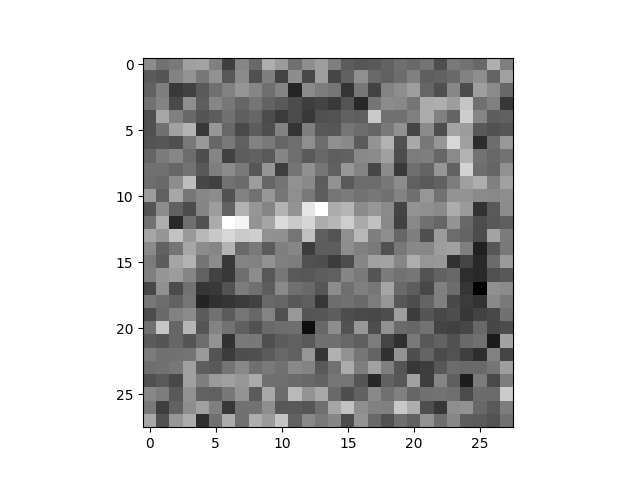
\includegraphics[width=0.25\linewidth]{co22.png}}
	\subfloat[588]{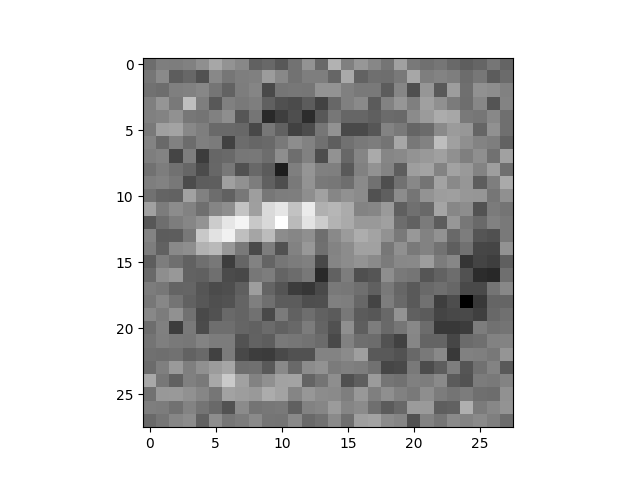
\includegraphics[width=0.25\linewidth]{co32.png}}
	\subfloat[Reg]{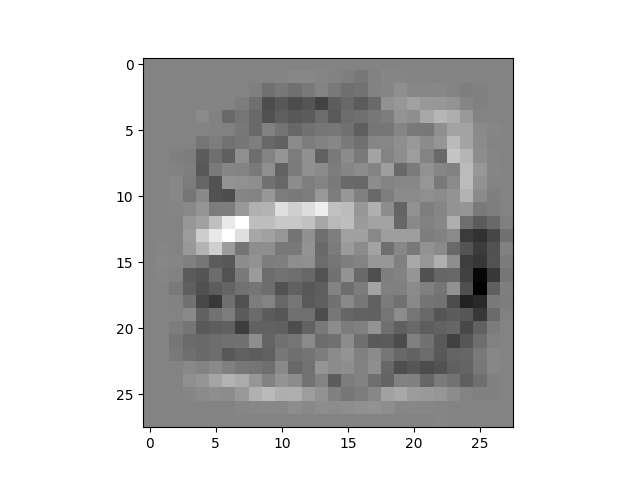
\includegraphics[width=0.25\linewidth]{reg2.png}}  
	\label{fig5} 
\end{figure}

\section*{Exponentiated Gradient Optimization}

\subsection*{Idea}

In this section, we explore the robustness of idential models trained using two optimizers: stochastic gradient descent and exponentiated gradient. Because the weights learned by each optimization scheme may be different, models trained using the two schemes may be more or less difficult to fool using adversarial noise. Additionally, attacks generated for one optimizer may not transfer to another.

The two optimizers may be compared in terms of what divergence we must choose to get their update rule.
Using squared difference as a divergence we arrive at the familiar gradient descent update rule:
$$ w_{t+1} \, \dot{=} \, w_t - \eta \nabla L(w_t). $$
The choice of relative entropy as a divergence (Kivinen, J \& Warmuth, M 1997) results in the following update rule, known as Exponentiated Gradient (EG):
$$ w_{t+1} \, \dot{=} \, w_t e^{-\eta \nabla L(w_t)}. $$
When extended to the case where weights can be negative, the above optimization scheme is known as EG plus/minus. We use this extension for training of neural networks in this section.

In this section, we investigate the robustness of models trained using each optimizer to adversarial attacks, and measure the transferability of attacks between said models.

\subsection*{Method}

In order to accurately compare the two optimizers, we train two initially identical networks to convergence using SGD and stochastic EG$\pm$. The architecture we chose for these experiments was a fully-connected neural network with a single hidden layer of 100 hidden nodes (FC 784-100-10).

After training, we generate adversarial attacks againsts each network using iterative fast gradient sign (FGS), and simple gradient ascent (GA) on the input image, both optimizing with respect to the negative correct score.

To compare robustness, we measure the number of iterations each method requires to fool each model. We then visualize the average perturbations needed to fool each network in order to gain insight into the network's internals, and compare transferability of equally strong attacks generated for each model.

In order to do fast experimentation, we implemented the EG$\pm$ optimizer and each adversarial attack method in PyTorch.

\begin{figure}
	\centering
	\caption{\enspace Adversarial attack samples generated using gradient ascent. From left to right, the columns are original image, noise to fool SGD-trained model, resulting adversarial example for SGD-trained model, noise to fool EG-trained model, resulting adversarial example generated for EG-trained model.}
	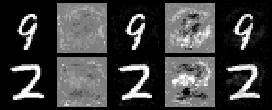
\includegraphics[width=\linewidth]{mnist_attacks.png}
	\label{fig6}
\end{figure}

\subsection*{Results}

In Table \ref{tab2}, we see that on average EG was $1.3\times$ more robust than SGD in terms of number of iterations taken to fool the models. To note is that it was significantly stronger against the fast gradient sign method, which distributes perturbations evenly across the image. This hints that the EG-trained model may have weak dependence on most of the pixels, relative to SGD which learns strong dependencies even on pixels which are rarely present.

\begin{table}
	\caption{\enspace Number of iterations to fool each model: mean($\pm$std)}
	\label{tab2}
	\begin{tabular*}{\hsize}{@{\extracolsep{\fill}}ccc}
		\hline
		\\[-7pt]
		\multicolumn{1}{c}{\it Method/Optimizer} & 
		\multicolumn{1}{c}{\it SGD}              & 
		\multicolumn{1}{c}{\it EG}               \\ 
		\hline
		\\[-5pt] 
		Gradient Ascent    & $60.9 (\pm 32.3)$ & $85.1 (\pm 40.5)$ \\ 
		Fast Gradient Sign & $52.0 (\pm 26.1)$ & $91.0 (\pm 43.5)$
	\end{tabular*}
\end{table}

Exploring this idea further, we visualized in Figure \ref{fig7} the average perturbation required to fool each model. We limit this visualization to the case of iterative gradient ascent to generate adversarial examples for input images labeled 3. The SGD-trained model is fooled largely by a collection of pixels on the periphery of the image, which are seldom if ever active in the training set. The EG$\pm$-trained model is undisturbed by these pixels, and requires a densely packed set of pixels concentrated in the difference between a three and an eight. It also effectively recovers the structure of the three, and is highly impacted by reductions to pixels in this structure. In contrast to SGD, the pixels which have a high impact on the score of the EG$\pm$-trained model make more semantic sense and are more likely to be activated in the training set.

\begin{figure}
	\centering
	\caption{\enspace Average fooling perturbation for threes, SGD (left) and EG$\pm$ (right).}
	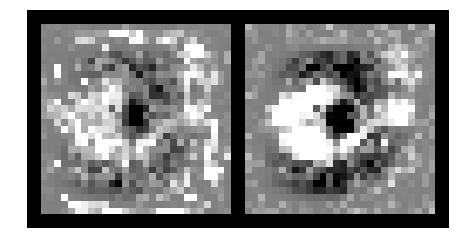
\includegraphics[width=\linewidth]{avg_attack_3.png}
	\label{fig7}
\end{figure}

Because EG$\pm$ is undisturbed by the same collection of peripheral pixels which are highly effective at fooling SGD, we expect that the transferability of attacks from SGD to EG$\pm$ will be low. In contrast, the structures present to fool EG$\pm$ are still weakly present in the average perturbation to fool SGD, so we expect the transferability of attacks from EG$\pm$ to SGD to be high. To test these hypotheses, we generated attacks for each optimizer using a fixed number of iterations. We then measured the transferability of attack from one optimizer to another. The results of this experiment are reported in Table \ref{tab3}, and confirm our hypothesis.

\begin{table}
	\caption{\enspace Percentage of successfully transferred attacks from one optimizer to the other.}
	\label{tab3}
	\begin{tabular*}{\hsize}{@{\extracolsep{\fill}}ccc}
		\hline
		\\[-7pt]
		\multicolumn{1}{c}{\it Method/ Src$\to$Dst} & 
		\multicolumn{1}{c}{\it SGD$\to$EG}          & 
		\multicolumn{1}{c}{\it EG$\to$SGD}          \\ 
		\hline
		\\[-5pt] 
		Gradient Ascent     & 67.4\% & 99.0\% \\
		Fast Gradient Sign  & 88.2\% & 99.8\%
	\end{tabular*}
\end{table}

In conclusion, EG$\pm$ has been demonstrated as more robust than SGD against adversarial attacks. Based on Figure \ref{fig6}, the weights learned by EG$\pm$ have higher semantic significance, which leads the model to be harder to fool using peripheral pixels. Because of this, attacks against SGD have a significantly lower transferability to EG$\pm$ than the other way around. For future experiments, we suggest comparing EG$\pm$ to L1-regularized SGD, which we expect may have similar properties.

\section*{Detection of Adversarial Examples using Reconstruction Error}

\subsection*{Idea}

To decrease overfitting, Capsule Networks are commonly trained alongside a reconstruction, or decoder network which uses the vector output from the highest probability final capsule to attempt to reconstruct the input image. In other words, the decoder receives vector output only from the capsule of the predicted class. The architecture of a capsule network is shown in Figure \ref{fig9}, but all that is needed to understand this experiment is that it follows an encoder-decoder structure where the encoder is also responsible for classification.

These output vectors have far less dimensionality than the input, and as a result the decoder network is limited to reconstructing images that lie on a low-dimensional manifold fit to the winning class only. Each digit class of MNIST lies near a low-dimensional manifold, so can typically be reconstructed with low loss. On the other hand, adversarial examples are close to the manifold of their original class, but the decoder will be forced to try to reconstruct them using the manifold for a different digit. As a result, we expect high reconstruction error. In the following section, we use the mean-squared error between the reconstructed image and input to detect adversarial examples, and report our results in the form of an ROC curve.

Because we generate attacks using gradients from the classification network, but do not use information from the decoder network, these attacks are generated in a scenario that is white-box with respect to the classification/encoder network, and black-box with respect to the decoder.

\begin{figure}[h!]
	\centering
	\caption{\enspace Capsule Network Architecture}
	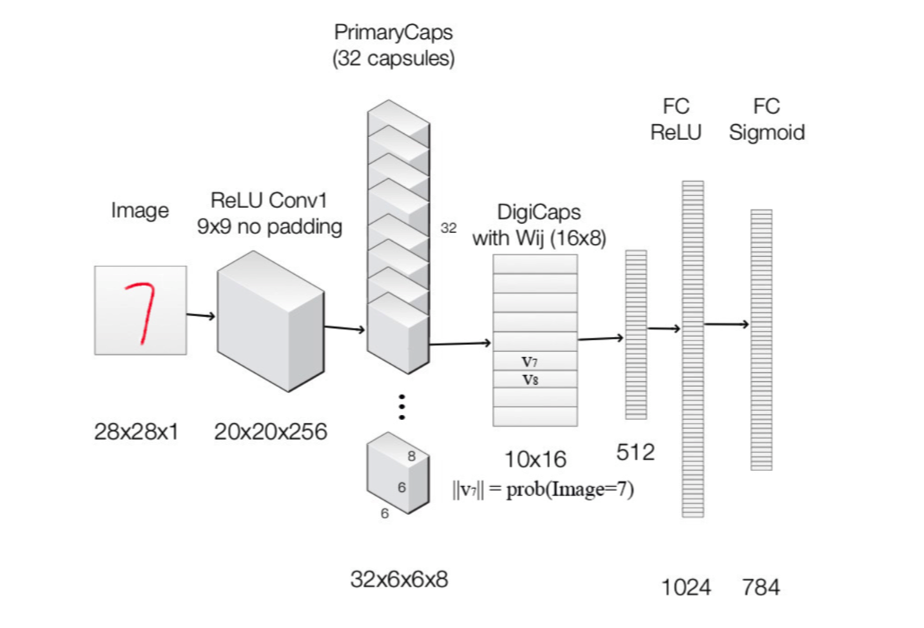
\includegraphics[width=\linewidth]{caps_recon}
	\label{fig9}
\end{figure}

\subsection*{Method}

After implementing the necessary models and utilities, this experiment was straightforward. First, we trained a capsule network for ten epochs on MNIST, achieving a test accuracy of 99.3\%. Further training was time-consuming and inconsequential for the purposes of adversarial attacks. We then ran the iterative gradient ascent method, as described in the previous section, to generate untargeted adversarial attacks for a subset of 1024 images. Lastly, we measure the mean-squared error for the reconstructions of each of these images and report the ROC curve of a linear threshold on this error to classify whether an input is adversarial.

As part of this experiment, we implemented a capsule network and utilities to measure reconstruction error in PyTorch. This code for this section and the previous can be found at \url{https://github.com/KellerJordan/CapsNet-Adversarial}.

\begin{figure}[h!]
	\centering
	\caption{\enspace Reconstruction of original and adversarial inputs. Columns from left: original image, reconstruction of original image, adversarial image, reconstruction of adversarial image}
	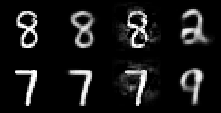
\includegraphics[width=\linewidth]{recon-fig5}
	\label{fig10}
\end{figure}

\begin{figure}[h!]
	\centering
	\caption{\enspace More examples. Columns as in Figure \ref{fig10}.}
	\subfloat[Network fooled to predict label 2]{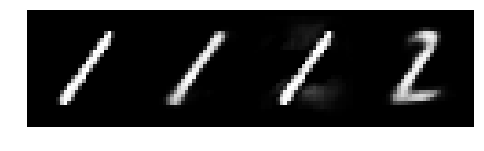
\includegraphics[width=\linewidth]{recon-fig4}} \\
	\subfloat[Network fooled to predict label 7]{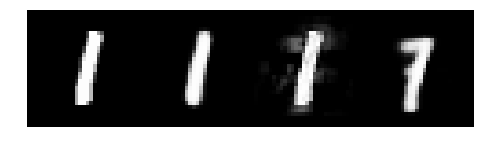
\includegraphics[width=\linewidth]{recon-fig3}}
	\label{fig11}
\end{figure}

\subsection*{Results}

In Figures \ref{fig10} and \ref{fig11} we observe that the network can effectively reconstruct natural inputs using the manifold corresponding to the unperturbed prediction, but fails to do so using the manifold for the class it was adversarially fooled into predicting. After recording the mean-squared error for a batch of 1024 adversarial and natural inputs, we report in Figure \ref{fig12} the ROC curve for a linear threshold classifying the inputs as adversarial or natural.

\begin{figure}[h!]
	\centering
	\caption{\enspace Receiving Operating Characteristic Curve for attack detection using different thresholds of MSE.}
	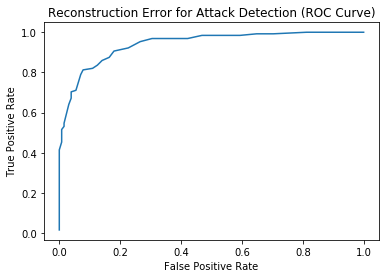
\includegraphics[width=\linewidth]{mse_roc}
	\label{fig12}
\end{figure}

At a false-positive rate of 5\%, this method can successfully detect nearly 70\% of adversarial examples. These results could be further improved by increasing the expressiveness of the decoder network and using a more effective loss function. As encoder-decoder architectures such as capsule networks become more widely adopted and usable in complex datasets, we believe that this technique will be an effective defense against adversarial attacks.

%\bibliographystyle{apalike}
%\bibliography{references.bib}

\section*{Bibliography}

Sara Sabour, Nicholas Frosst, and Geoffrey E Hinton. \textit{Dynamic routing between capsules}. In
Advances in Neural Information Processing Systems, pp. 3859–3869, 2017.

Kivinen, J \& Warmuth, M (1997). \textit{Additive versus exponentiated gradient updates for linear
prediction}. Journal of Tnformation and Computation 132, 1-64. 


\end{document}




